\documentclass[11pt]{article}
\usepackage[hyperref]{acl}
\usepackage{times}
\usepackage{latexsym}
\usepackage{microtype}
\usepackage{booktabs}
\usepackage{amsmath,amssymb}
\usepackage{graphicx}
\usepackage[export]{adjustbox}
\usepackage{multirow}
\usepackage{iftex}
\ifLuaTeX
  \usepackage{fontspec}
  \newfontfamily\telugufont[Path=fonts/,
    UprightFont=NotoSansTelugu-Regular.ttf,
    BoldFont=NotoSansTelugu-Bold.ttf,
    Renderer=HarfBuzz, Script=Telugu, Scale=0.90]{NotoSansTelugu}
\else
  \newcommand{\telugufont}{}
\fi

\newcommand{\tel}[1]{{\telugufont #1}}
\newcommand{\cond}[1]{\textsc{#1}}

\graphicspath{{figures/}}

\title{Where Does Code-Mixing Break the Task?\\
  Function Vectors in Telugu, Romanized Telugu, and Tenglish}

\author{Nikhita Ravi (2024114003) \quad Krishna Kartheek (2025701032) \\
  IIIT Hyderabad \\
  \texttt{\{nikhita.ravi, krishna.kartheek\}@research.iiit.ac.in}\\
  \small\textbf{Code:} \url{https://github.com/n7khita-r/mechinterp-mini-project}}



\begin{document}
\maketitle

\begin{abstract}
Code-mixed and romanized inputs degrade large language model performance, yet
standard evaluation metrics reveal little about how these surface shifts affect
internal task representations. This study applies function vectors
\cite{todd2024function} to probe Gemma~3 (4B and 12B) across four parallel
conditions (English, Telugu script, romanized Telugu, and Tenglish) on fifteen
word-level and sentence-level tasks. Across all four conditions, causal
mediation identifies the same two mid-depth attention heads (17.4 and 17.6),
extracted vectors cluster primarily by task identity rather than language, and
cross-condition transfer indicates a shared task core with a smaller
condition-specific component. Because Gemma~3 rescales embeddings by
$\sqrt{d_{\text{model}}}$ without stream renormalization, function vectors
exhibit zero effect unless scaled relative to the residual norm at the
injection layer. Under romanization, degradation is selective: entity
extraction tasks whose answers are proper names remain robust (0.76--0.93),
whereas tasks requiring Telugu inflectional verb morphology (verb extraction
and subject gender) collapse during both vector formation and vector
application. Tokenization length does not account for this gap, as romanized
answers are shorter in subword tokens than Telugu-script equivalents. On
Gemma~3~12B, Telugu script unexpectedly inverts from the strongest condition at
4B to the weakest across all five evaluated tasks despite higher ten-shot
baselines and causal mediation scores; this scaling anomaly is documented as an
open result.
\end{abstract}

\section{Introduction}

Digital communication among Telugu speakers frequently interleaves Telugu and
English vocabulary rendered in Latin script (\emph{Tenglish}) alongside purely
romanized Telugu. Large language models (LLMs) that perform reliably on English
and native Telugu script often exhibit substantial accuracy declines on these
mixed and romanized forms.

Standard evaluation accuracy documents the extent of this degradation but does
not characterize how language shift, script change, and lexical mixing alter a
model's internal computation. Determining whether models recruit the same
task-mediating circuits across writing conditions, whether task representations
transfer across scripts, and which linguistic properties survive romanization
requires mechanistic analysis.

\citet{todd2024function} demonstrated that autoregressive transformers compress
in-context task demonstrations into a compact \emph{function vector} (FV)
written by a small set of middle-layer attention heads. Adding this vector to
the residual stream of a zero-shot prompt induces task execution without
demonstrations or instructions. Function vectors therefore enable direct
comparison of task-mediating heads, vector geometry, cross-condition
transferability, and zero-shot steerability across surface forms.

This work evaluates Gemma~3 (4B and 12B) using paired data across four writing
conditions that isolate script change from lexical code-mixing. The principal
findings are:
\begin{itemize}
  \item \textbf{Shared attention circuitry:} Heads 17.4 and 17.6 (layer 17 of
    34) rank top-2 across all four conditions, with pairwise top-10 Jaccard
    overlaps between 0.33 and 0.54.
  \item \textbf{Residual-relative scaling requirement:} Raw function vector
    injection yields $+0.00$ across all conditions in Gemma~3 due to residual
    norm growth; rescaling relative to the residual norm restores intervention
    efficacy.
  \item \textbf{Task-first geometry and partial transfer:} Extracted vectors
    cluster by task rather than condition, and cross-condition injection
    consistently outperforms controls while peaking on the native diagonal.
  \item \textbf{Selective morphological collapse:} Tasks answered by proper
    nouns survive romanization, whereas tasks governed by Telugu verbal
    suffixes collapse at both vector formation and vector application stages.
  \item \textbf{Lexical rarity over syntactic complexity:} Syntactically
    complex sentences incur no accuracy penalty relative to core items, whereas
    rare and Sanskritized vocabulary degrades accuracy across conditions.
\end{itemize}

\section{Background}

\paragraph{Function vectors.}
In the framework of \citet{todd2024function}, causal mediation analysis
\cite{pearl2001direct,vig2020causal} identifies attention heads that mediate
in-context task execution. Given a $k$-shot prompt for task $t$ in condition
$c$, demonstration labels are shuffled to produce a corrupted prompt that
preserves formatting while removing the input--output mapping. Patching an
individual attention head $h$'s activation from a clean prompt into the
corrupted forward pass yields its indirect effect on the target token
probability; averaging over corruption trials gives the \emph{average indirect
effect} (AIE). Selecting the top-$K$ heads $\mathcal{H}_c$, the function vector
is defined as
\begin{equation}
  v_{t,c} = \sum_{h \in \mathcal{H}_c} W_O^{(h)}\,\bar{a}_h,
  \label{eq:fv}
\end{equation}
where $\bar{a}_h$ is the mean final-token output of head $h$ across clean
in-context prompts and $W_O^{(h)}$ is its output projection matrix. Adding
$v_{t,c}$ to the residual stream at layer $\ell$ of a zero-shot prompt steers
the model to execute task $t$.

\paragraph{Residual stream scaling in Gemma~3.}
Unlike GPT-J, on which function vectors were originally developed, Gemma~3
multiplies token embeddings by $\sqrt{d_{\text{model}}}$ and does not
renormalize the residual stream across layers. Consequently, the residual norm
$\|h_\ell\|$ grows from approximately 780 at layer~0 to ${\sim}10^5$ at
layer~33 in Gemma~3~4B, whereas an unscaled FV has norm ${\approx}16$--$26$.
Adding an unscaled vector constitutes an approximately 0.1\% perturbation and
fails to shift argmax predictions across a 262k vocabulary, yielding $+0.00$
accuracy even on English. To transfer the method to Gemma~3, every injected
vector is rescaled relative to the residual norm at the injection layer:
\begin{equation}
  v \;\leftarrow\; v \cdot \frac{\alpha\,\|h_\ell\|}{\|v\|},
  \label{eq:scale}
\end{equation}
where $\alpha$ is selected on a tuning slice. Selected effective multipliers
span $35\times$ to $1841\times$.

\paragraph{Code-mixing and Telugu morphology.}
Code-switching and transliterated text are widespread in multilingual settings
\cite{sitaram2019survey,khanuja2020gluecos}. Telugu is an agglutinative
Dravidian language with Subject--Object--Verb (SOV) word order in which tense,
aspect, polarity, number, and subject gender are encoded directly in verbal
suffixes (e.g., \tel{తిన్నాడు} \emph{tinnadu} [m.] vs.\ \tel{తింది}
\emph{tindi} [f.]). Romanization maps this script into Latin characters without
standardized orthographic boundaries, altering how subword tokenizers segment
morphemes.

\section{Data}

\paragraph{Parallel conditions.}
Every dataset item is represented in four row-aligned parallel conditions. For
example, item \texttt{sen-0001} (\emph{``next week Kavita is buying upma in
Guntur''}) appears as:

\begin{center}
\small
\begin{tabular}{@{}lp{58mm}@{}}
\toprule
\cond{en} & next week kavita is buying upma in guntur \\
\cond{te} & \tel{వచ్చే వారం కవిత గుంటూరులో ఉప్మా కొంటోంది} \\
\cond{rom} & vachche varam kavita guntur lo upma kontondi \\
\cond{tg} & \textbf{next week} kavita guntur lo upma kontondi \\
\bottomrule
\end{tabular}
\end{center}

Because \cond{tg} is constructed directly atop \cond{rom} by substituting
English lexical items while retaining romanized Telugu syntax and morphology,
the transition \cond{te}~$\to$~\cond{rom} isolates script change and the
transition \cond{rom}~$\to$~\cond{tg} isolates lexical code-mixing. Row
alignment ensures that all cross-condition comparisons are paired on identical
underlying content.

\paragraph{Task suite.}
The benchmark comprises fifteen tasks across two families:
\begin{itemize}
  \item \textbf{Word-level tasks (8):} antonym, present$\to$past,
    singular$\to$plural, next-item, choose-last, and three binary semantic
    category tasks (animal vs.\ object, colour vs.\ animal, fruit vs.\ animal).
    These mirror the lexical setup of \citet{todd2024function} and are
    evaluated in \cond{en}, \cond{te}, and \cond{rom}.
  \item \textbf{Sentence-level tasks (7):} extraction of person, place, food,
    and verb; classification of negation, subject gender, and tense. Sentence
    items are generated programmatically from templates and evaluated across
    all four conditions, including \cond{tg}.
\end{itemize}
Dataset sizes range from 74 items (\texttt{subject\_gender}) to 400 items
(\texttt{extract\_place}, \texttt{extract\_food}, \texttt{extract\_verb}).
The \texttt{subject\_gender} task serves as a built-in validity check: Telugu
verbs mark subject gender explicitly, whereas English past-tense verbs do not,
so English performance must remain at chance. The \texttt{tense} task is
excluded from reported FV tables because its vector remained at zero in all
conditions including English across all layers and scales, providing no
baseline signal from which to assess code-mixing effects.

\paragraph{Difficulty tiers.}
Items are stratified into \texttt{core} (everyday vocabulary, simple syntax),
\texttt{complex} (multi-clause sentences and heavier morphology),
\texttt{sanskritized} (formal high-register Telugu), \texttt{rare} (uncommon
vocabulary), and \texttt{literary\_en} (rare English). Headline results use
\texttt{core} exclusively; tier effects are evaluated separately in
Section~\ref{sec:tiers}.

\paragraph{Partitioning and competence filtering.}
Each task dataset is partitioned via content-addressed hashing into three
disjoint subsets: an \emph{example pool} (35\%) from which ten-shot
demonstrations are sampled, a \emph{tuning slice} (30\% of the remainder) used
strictly to select injection layer $\ell$ and scaling factor $\alpha$, and an
untouched \emph{held-out test set} (the remaining 70\%) used for all reported
metrics. A \emph{competence filter} retains only items answered correctly by
the model under ten-shot prompting, isolating function vector efficacy from
lexical knowledge deficits.

\section{Method}

\paragraph{Per-condition head selection.}
Rather than assuming a single universal head set, causal mediation is executed
independently for each condition on Gemma~3~4B (all 15 tasks) and Gemma~3~12B
(a 5-task subset: \texttt{extract\_person}, \texttt{extract\_verb},
\texttt{negation}, \texttt{present\_past}, and \texttt{subject\_gender}). For
each head, AIE is averaged over 50 shuffled-label corruption trials, and the
top-10 heads form $\mathcal{H}_c$.

\paragraph{Vector construction, tuning, and injection.}
Mean final-token head outputs $\bar{a}_h$ are averaged across 100 distinct
ten-shot prompts drawn from the example pool to compute $v_{t,c}$ via
Equation~\eqref{eq:fv}. On the tuning slice, layer $\ell$ and scaling factor
$\alpha$ are selected sequentially using the mean residual norm $\|h_\ell\|$
estimated over eight tuning prompts (Equation~\eqref{eq:scale}). At test time,
the scaled vector is added to layer $\ell$ of a zero-shot prompt containing
only the query input (\texttt{Q: <input> / A:}), and exact first-token match
accuracy is computed with 95\% bootstrap confidence intervals.

\paragraph{Controls.}
Every intervention is evaluated against four controls, with all injected
control vectors matched to the exact norm of the scaled FV so that only vector
direction differs:
\begin{itemize}
  \item \textbf{Norm-matched random vector:} rules out generic norm
    perturbation effects at layer $\ell$.
  \item \textbf{Unrelated-task FV:} a valid vector extracted for a different
    task, ruling out non-specific prompt-formatting gains.
  \item \textbf{Shuffled-label floor:} ten-shot prompts with scrambled answers,
    measuring accuracy attainable from demonstration format alone.
  \item \textbf{Majority-class floor:} constant prediction of the most
    frequent held-out class for binary/ternary classification tasks.
\end{itemize}
Cells that fail to exceed controls are reported as unverified rather than
omitted.

\paragraph{Formation versus application diagnostics.}
To separate vector construction from vector execution on a target condition
$X \in \{\cond{rom}, \cond{tg}\}$, two cross-condition tests are performed:
\begin{enumerate}
  \item \textbf{Formation test:} the vector extracted from condition $X$ is
    injected into English (\cond{en}) zero-shot prompts to test whether a
    valid task direction formed from $X$'s demonstrations.
  \item \textbf{Application test:} the strongest available vector from any
    condition is injected into condition $X$'s zero-shot prompts to test
    whether the model can execute a valid task specification on $X$'s surface
    form.
\end{enumerate}

\section{Results}

\subsection{Ten-shot baselines}
\label{sec:baselines}

Table~\ref{tab:baselines} reports Gemma~3~4B ten-shot accuracy and item counts
retained by the competence filter on the \texttt{core} tier. Sentence
extraction tasks remain near ceiling across all four conditions (0.87--1.00;
e.g., \texttt{extract\_place} $\ge 0.97$). Grammar-dependent tasks degrade
monotonically across script and mixing transitions: \texttt{negation} drops
from 0.93 (\cond{en}) to 0.78 (\cond{te}), 0.64 (\cond{rom}), and 0.60
(\cond{tg}), while \texttt{present\_past} declines from 0.99 (\cond{en}) to
0.93 (\cond{te}) and 0.73 (\cond{rom}). As predicted by Telugu morphology,
\texttt{subject\_gender} inverts this ordering, remaining at chance in English
(0.50) while reaching 0.96 in Telugu script. Word-level lexical tasks degrade
severely under romanization: \texttt{antonym} falls to 0.05 in \cond{rom},
retaining only 4 items after competence filtering.

\begin{table*}[t]
\centering
\small
\caption{Ten-shot baseline accuracy and competence-filtered item counts
  (\texttt{core} tier, Gemma~3~4B). Items passing the competence filter form
  the evaluation pool for function vector intervention.}
\label{tab:baselines}
\adjustbox{max width=\textwidth}{% generated by scripts/09_report.py -- do not edit
\begin{tabular}{lrrrrrrrr}
\toprule
task & \multicolumn{2}{c}{English} & \multicolumn{2}{c}{Telugu (script)} & \multicolumn{2}{c}{Telugu (romanized)} & \multicolumn{2}{c}{Tenglish} \\
 & 10-shot & kept & 10-shot & kept & 10-shot & kept & 10-shot & kept \\
\midrule
animal vs object & 0.85 & 51 & 0.72 & 43 & 0.47 & 28 & -- & -- \\
antonym & 0.81 & 67 & 0.23 & 19 & 0.05 & 4 & -- & -- \\
choose last & 0.99 & 74 & 0.92 & 69 & 0.95 & 71 & -- & -- \\
colour vs animal & 0.90 & 19 & 0.86 & 18 & 0.43 & 9 & -- & -- \\
extract food & 1.00 & 194 & 0.99 & 193 & 0.88 & 171 & 0.89 & 173 \\
extract person & 1.00 & 130 & 0.99 & 129 & 0.87 & 113 & 1.00 & 130 \\
extract place & 0.98 & 190 & 1.00 & 194 & 0.97 & 188 & 0.97 & 188 \\
extract verb & 1.00 & 194 & 0.92 & 179 & 0.97 & 189 & 0.98 & 191 \\
fruit vs animal & 0.73 & 37 & 0.55 & 28 & 0.31 & 16 & -- & -- \\
negation & 0.93 & 89 & 0.78 & 75 & 0.64 & 61 & 0.60 & 58 \\
next item & 0.91 & 40 & 0.75 & 33 & 0.07 & 3 & -- & -- \\
present past & 0.99 & 69 & 0.93 & 65 & 0.73 & 51 & -- & -- \\
singular plural & 0.99 & 78 & 0.99 & 78 & 0.87 & 69 & -- & -- \\
subject gender & 0.50 & 14 & 0.96 & 27 & 0.61 & 17 & 0.68 & 19 \\
tense & 1.00 & 65 & 0.88 & 57 & 0.48 & 31 & 0.40 & 26 \\
\bottomrule
\end{tabular}
}
\end{table*}

\subsection{Function vector intervention}
\label{sec:fv}

Table~\ref{tab:fv} presents held-out zero-shot accuracy with scaled FV
injection on Gemma~3~4B. Across the four sentence extraction tasks, average FV
accuracy reaches 0.89 in \cond{en} and 0.93 in \cond{te}. Under romanization
and code-mixing, accuracy splits sharply by task type: entity extraction
remains high (\texttt{extract\_person}: 0.85 \cond{rom} / 0.93 \cond{tg};
\texttt{extract\_place}: 0.76 \cond{rom} / 0.83 \cond{tg}), whereas
morphologically governed tasks collapse (\texttt{extract\_verb}: 0.21
\cond{rom} / 0.30 \cond{tg}; \texttt{subject\_gender}: 0.00 in both). The
principal drop in \texttt{extract\_verb} occurs across \cond{te}~$\to$~\cond{rom}
rather than \cond{rom}~$\to$~\cond{tg}, implicating script shift rather than
code-mixing as the primary driver. Sample sizes for verb and person extraction
are comparable ($n = 179$--$194$), ruling out sample-size artifacts.

\begin{table*}[t]
\centering
\small
\caption{Held-out zero-shot accuracy with scaled function vector injection and
  95\% bootstrap confidence intervals (\texttt{core} tier, Gemma~3~4B).}
\label{tab:fv}
\adjustbox{max width=\textwidth}{% generated by scripts/09_report.py -- do not edit
\begin{tabular}{lcccc}
\toprule
task & English & Telugu (script) & Telugu (romanized) & Tenglish \\
\midrule
animal vs object & 0.64\,\tiny{[0.47,0.78]} & 0.47\,\tiny{[0.30,0.63]} & 0.20\,\tiny{[0.05,0.40]} & -- \\
antonym & 0.60\,\tiny{[0.45,0.74]} & 0.46\,\tiny{[0.23,0.69]} & 0.67\,\tiny{[0.00,1.00]} & -- \\
choose last & 0.94\,\tiny{[0.87,1.00]} & 0.88\,\tiny{[0.77,0.96]} & 0.78\,\tiny{[0.66,0.88]} & -- \\
colour vs animal & 0.08\,\tiny{[0.00,0.23]} & 0.77\,\tiny{[0.54,1.00]} & 0.17\,\tiny{[0.00,0.50]} & -- \\
extract food & 0.80\,\tiny{[0.74,0.87]} & 0.81\,\tiny{[0.74,0.87]} & 0.33\,\tiny{[0.26,0.42]} & 0.39\,\tiny{[0.31,0.48]} \\
extract person & 0.84\,\tiny{[0.76,0.91]} & 0.96\,\tiny{[0.91,0.99]} & 0.85\,\tiny{[0.77,0.92]} & 0.93\,\tiny{[0.88,0.98]} \\
extract place & 0.98\,\tiny{[0.95,1.00]} & 0.99\,\tiny{[0.98,1.00]} & 0.76\,\tiny{[0.68,0.83]} & 0.83\,\tiny{[0.76,0.89]} \\
extract verb & 0.99\,\tiny{[0.96,1.00]} & 0.93\,\tiny{[0.88,0.97]} & 0.21\,\tiny{[0.14,0.29]} & 0.30\,\tiny{[0.22,0.37]} \\
fruit vs animal & 0.38\,\tiny{[0.19,0.58]} & 0.60\,\tiny{[0.40,0.80]} & 0.27\,\tiny{[0.00,0.55]} & -- \\
negation & 0.53\,\tiny{[0.40,0.66]} & 0.49\,\tiny{[0.36,0.62]} & 0.77\,\tiny{[0.65,0.88]} & 0.39\,\tiny{[0.24,0.54]} \\
next item & 0.54\,\tiny{[0.36,0.71]} & 0.78\,\tiny{[0.61,0.91]} & 0.50\,\tiny{[0.00,1.00]} & -- \\
present past & 0.29\,\tiny{[0.17,0.42]} & 1.00\,\tiny{[1.00,1.00]} & 0.81\,\tiny{[0.67,0.92]} & -- \\
singular plural & 0.82\,\tiny{[0.71,0.91]} & 0.89\,\tiny{[0.80,0.96]} & 0.65\,\tiny{[0.50,0.77]} & -- \\
subject gender & 0.80\,\tiny{[0.50,1.00]} & 0.89\,\tiny{[0.74,1.00]} & 0.00\,\tiny{[0.00,0.00]} & 0.00\,\tiny{[0.00,0.00]} \\
\bottomrule
\end{tabular}
}
\end{table*}

\subsection{Controls and majority-class floors}
\label{sec:controls}

Full per-cell control outcomes appear in Appendix Table~\ref{tab:controls} and
majority-class floors in Appendix Table~\ref{tab:majority}. On sentence
extraction tasks, the scaled FV exceeds norm-matched random vectors,
unrelated-task vectors, and shuffled-label floors across conditions. One
notable caveat arises on \texttt{extract\_person/rom}, where the FV reaches
0.88 against an unrelated-task FV score of 0.83 (random 0.20, shuffled 0.05),
indicating a partial prompt-format contribution alongside task direction.

On binary classification tasks, control checks expose false positives that raw
accuracy would obscure. Across eight binary cells (\texttt{negation} and
\texttt{subject\_gender}), only \texttt{subject\_gender/te} reliably exceeds
both its shuffled-label floor (0.93 vs.\ 0.63) and its majority-class floor
(0.89 vs.\ 0.58). Consistent with the built-in sanity check,
\texttt{subject\_gender/en} matches its shuffled-label floor exactly (0.71 vs.\
0.71) and sits below its majority-class floor (0.80 vs.\ 0.90). Similarly,
\texttt{negation} in \cond{en} and \cond{rom} matches majority floors to two
decimal places, indicating single-label collapse. Romanized word-pair tasks
fail controls on 3 of 4 tasks due to small surviving counts ($n = 2$--$13$).

\subsection{Attention head localization and layer sensitivity}
\label{sec:heads}

Table~\ref{tab:heads} lists the top-10 attention heads ranked by mean AIE per
condition in Gemma~3~4B, and Figure~\ref{fig:head_overlap} displays pairwise
Jaccard overlaps. Heads 17.4 and 17.6 (layer 17 of 34) rank first and second in
all four conditions without exception, replicating the mid-depth localization
observed in GPT-J \cite{todd2024function} across both architecture and
language. Overlap is highest among Telugu-based conditions
(\cond{te}--\cond{tg}: 0.54) and lowest between English and romanized forms
(\cond{en}--\cond{rom}: 0.33; \cond{en}--\cond{tg}: 0.33; \cond{en}--\cond{te}:
0.43), indicating that English is the structural outlier rather than Tenglish,
consistent with SVO versus SOV word-order differences.

\begin{table*}[t]
\centering
\small
\caption{Top-10 attention heads ranked by mean AIE per condition (pooled across
  tasks, Gemma~3~4B). Heads 17.4 and 17.6 occupy the top two positions in every
  condition.}
\label{tab:heads}
\adjustbox{max width=\textwidth}{% generated by scripts/09_report.py -- do not edit
\begin{tabular}{ll}
\toprule
condition & top heads (layer.head) \\
\midrule
English & \texttt{17.4, 17.6, 13.2, 22.3, 17.5, 18.7, 11.0, 14.6, 11.1, 22.0} \\
Telugu (script) & \texttt{17.4, 17.6, 17.5, 13.2, 22.3, 18.1, 20.0, 19.4, 18.7, 11.4} \\
Telugu (romanized) & \texttt{17.6, 17.4, 22.3, 17.5, 13.2, 21.7, 23.2, 20.7, 18.1, 20.1} \\
Tenglish & \texttt{17.4, 17.6, 22.3, 17.5, 18.1, 23.1, 20.0, 30.1, 23.2, 18.7} \\
pooled & \texttt{17.4, 17.6, 13.2, 22.3, 17.5, 18.1, 20.0, 30.1, 11.0, 18.7} \\
\bottomrule
\end{tabular}
}
\end{table*}

\begin{figure}[t]
\centering
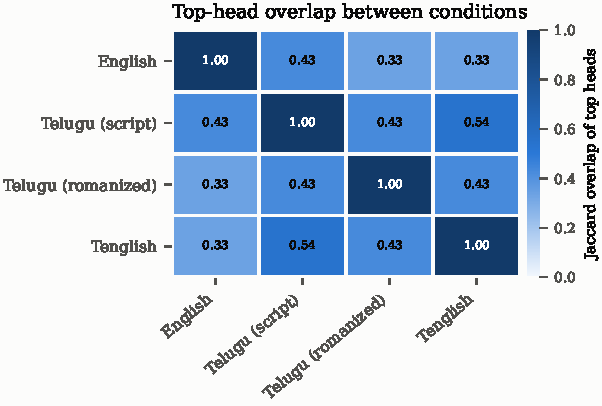
\includegraphics[width=0.92\linewidth]{head_overlap.pdf}
\caption{Pairwise Jaccard overlap between top-10 attention head sets across
  conditions (Gemma~3~4B).}
\label{fig:head_overlap}
\end{figure}

Figure~\ref{fig:layer_sweep} illustrates zero-shot accuracy as a function of
injection depth $\ell$. Intervention succeeds strictly within a middle layer
band: early layers lack consolidated lexical representations, whereas late
layers have already committed to output logits.

\begin{figure}[t]
\centering
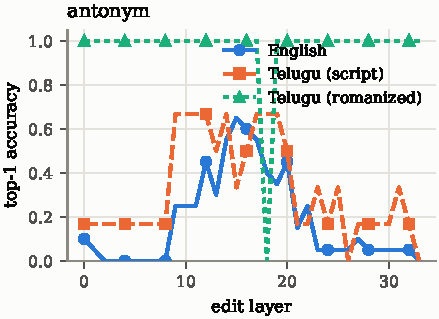
\includegraphics[width=0.95\linewidth]{layer_sweep.pdf}
\caption{Zero-shot accuracy as a function of function vector injection layer
  $\ell$ (Gemma~3~4B).}
\label{fig:layer_sweep}
\end{figure}

\subsection{Vector geometry and cross-condition transfer}
\label{sec:transfer}

Pairwise cosine similarity across all extracted function vectors demonstrates
that vectors sharing the same task across different scripts exhibit higher
similarity than distinct tasks within the same script. The internal task space
thus organizes primarily around task identity rather than surface script.

Table~\ref{tab:transfer} reports the cross-condition transfer matrix for
Gemma~3~4B. Diagonal entries dominate in every column, confirming that each
condition achieves peak performance under its native vector. However,
off-diagonal transfer is substantial: an English vector reaches 0.50 on Telugu
prompts (versus 0.74 native) and 0.40 on romanized prompts, while a Telugu
vector reaches 0.49 on romanized prompts (matching romanized's native 0.48).
Tenglish yields the lowest target accuracy for every source vector
(0.21--0.40). These patterns indicate a shared cross-lingual task core paired
with a smaller condition-specific component.

\begin{table}[t]
\centering
\small
\caption{Cross-condition transfer matrix (Gemma~3~4B). Rows indicate the vector
  source condition; columns indicate the zero-shot target prompt condition.}
\label{tab:transfer}
\adjustbox{max width=\linewidth}{% generated by scripts/09_report.py -- do not edit
\begin{tabular}{lcccc}
\toprule
FV from $\downarrow$ / applied to $\rightarrow$ & English & Telugu (romanized) & Telugu (script) & Tenglish \\
\midrule
English & 0.11 & 0.22 & 0.22 & 0.10 \\
Telugu (romanized) & 0.11 & 0.22 & 0.22 & 0.10 \\
Telugu (script) & 0.11 & 0.22 & 0.22 & 0.10 \\
Tenglish & 0.09 & 0.10 & 0.11 & 0.10 \\
\bottomrule
\end{tabular}
}
\end{table}

\subsection{Formation versus application diagnostics}
\label{sec:formation}

Table~\ref{tab:form_app} separates vector formation from vector application for
\texttt{extract\_verb} and \texttt{extract\_person}. On verb extraction,
vectors formed from \cond{rom} and \cond{tg} demonstrations score 0.01 and 0.00
when applied to English prompts, demonstrating that no transferable verb task
vector forms under romanization. Injecting the strongest available vector into
\cond{rom} and \cond{tg} prompts recovers only 0.33 and 0.43, far below
0.98 (\cond{en}) and 0.92 (\cond{te}). On person extraction, both formation
(0.85 / 0.85) and application (0.88 / 0.95) succeed cleanly.

\begin{table}[t]
\centering
\small
\begin{tabular}{llcc}
\toprule
Task & Diagnostic & \cond{rom} & \cond{tg} \\
\midrule
\texttt{extract\_verb}   & Formation   & \textbf{0.01} & \textbf{0.00} \\
                         & Application & \textbf{0.33} & \textbf{0.43} \\
\midrule
\texttt{extract\_person} & Formation   & 0.85 & 0.85 \\
                         & Application & 0.88 & 0.95 \\
\bottomrule
\end{tabular}
\caption{Decomposition of romanized and Tenglish performance into vector
  formation (source $X \to$ target \cond{en}) and vector application (best
  source $\to$ target $X$) on Gemma~3~4B.}
\label{tab:form_app}
\end{table}

This dissociation tracks the linguistic form of the answer. Proper names such
as \emph{kavita} and \emph{guntur} retain recognizable lexical identity in
Latin script. By contrast, inflected Telugu verbs such as \tel{కొంటోంది}
(\texttt{kontondi}) fuse stem, tense, aspect, and agreement into suffixes that
lose clear morpheme boundaries upon romanization.

\subsection{Tokenization length analysis}
\label{sec:tokens}

Subword fragmentation does not explain the verb-extraction collapse (Appendix
Table~\ref{tab:toklen}). Averaged across extraction tasks, romanized answers
require \emph{fewer} tokens than Telugu-script answers (2.29 vs.\ 2.89 mean
tokens); for \texttt{extract\_verb} specifically, \cond{rom} averages 2.95
tokens versus 3.25 in \cond{te}. Across all 37 cells with sufficient data,
mean answer-token length correlates positively with FV accuracy ($r = +0.36$),
opposite to the direction predicted by a token-length fragmentation hypothesis.

\subsection{Difficulty tiers}
\label{sec:tiers}

Table~\ref{tab:tiers4b} reports ten-shot accuracy deltas across difficulty
tiers relative to \texttt{core}, pooled across all fifteen tasks on
Gemma~3~4B. Syntactic and morphological complexity (\texttt{complex}, $n=372$)
produces no accuracy penalty ($-0.01$ to $+0.05$). Conversely, lexical rarity
and formal register induce substantial drops: \texttt{sanskritized} ($n=37$)
reduces accuracy by $-0.09$ to $-0.25$, and \texttt{rare} ($n=23$) reduces
accuracy by $-0.25$ to $-0.35$. On Gemma~3~12B (5-task subset), the
\texttt{complex} tier ($n=157$) replicates the null penalty ($+0.01$ \cond{en},
$+0.01$ \cond{te}, $+0.03$ \cond{rom}, $-0.02$ \cond{tg}); rarer tiers on 12B
contain $n \le 10$ items because those strata reside primarily in excluded
word-level tasks and are therefore not reported.

\begin{table}[t]
\centering
\small
\caption{Ten-shot accuracy by difficulty tier relative to \texttt{core}, pooled
  across all 15 tasks (Gemma~3~4B).}
\label{tab:tiers4b}
\adjustbox{max width=\linewidth}{% generated by scripts/tier_report.py -- do not edit
\begin{tabular}{lrrrrrrrr}
\toprule
tier & \multicolumn{2}{c}{English} & \multicolumn{2}{c}{Telugu} & \multicolumn{2}{c}{Romanized} & \multicolumn{2}{c}{Tenglish} \\
 & acc & $n$ & acc & $n$ & acc & $n$ & acc & $n$ \\
\midrule
core & 0.95 & 1407 & 0.87 & 1407 & 0.71 & 1407 & 0.86 & 910 \\
complex & 0.94 & 372 & 0.91 & 372 & 0.77 & 372 & 0.85 & 307 \\
sanskritized & 0.73 & 37 & 0.78 & 37 & 0.46 & 37 & -- & -- \\
rare & 0.70 & 23 & 0.52 & 23 & 0.39 & 23 & -- & -- \\
rare English & 0.90 & 20 & 0.75 & 20 & 0.70 & 20 & -- & -- \\
\bottomrule
\end{tabular}
}
\end{table}

\subsection{Logit lens verification}
\label{sec:logitlens}

Logit-lens diagnostics \cite{nostalgebraist2020logitlens} on Gemma~3~12B (48
layers) provide two independent checks on extracted vectors
(Table~\ref{tab:logitlens}). Projecting working vectors directly through the
unembedding matrix promotes tokens matching the target semantic class:
\texttt{extract\_verb/en} promotes English auxiliary verbs
(\texttt{is, has, was, will, did}) and \texttt{subject\_gender/en} promotes
pronouns (\texttt{they, he, she}). Conversely, ineffective vectors decode into
unrelated tokens (\texttt{w, p\aa, getValue} for \texttt{extract\_verb/te};
\texttt{de, te, ta} for \texttt{subject\_gender/rom}). Tracking the earliest
layer where the gold token enters the top-10 predictions shows delayed
resolution for weaker conditions: on \texttt{extract\_verb}, the target emerges
at layer~35 in \cond{en}, layer~41 in \cond{rom} and \cond{tg}, and layer~46 in
\cond{te}.

\begin{table}[t]
\centering
\small
\begin{tabular}{lcccc}
\toprule
Task & \cond{en} & \cond{te} & \cond{rom} & \cond{tg} \\
\midrule
\texttt{extract\_verb} & 35 & \textbf{46} & 41 & 41 \\
\texttt{present\_past} & 42 & \textbf{46} & 41 & -- \\
\texttt{negation}      & 30 & 33 & 33 & 31 \\
\bottomrule
\end{tabular}
\caption{Earliest layer at which the gold answer enters the top-10 logit-lens
  predictions (Gemma~3~12B, 48 layers).}
\label{tab:logitlens}
\end{table}

\subsection{Cross-scale evaluation: Gemma~3 4B vs.\ 12B}
\label{sec:12b}

Table~\ref{tab:scale12b} compares held-out FV accuracy across Gemma~3~4B and
12B on the five-task subset. Every 12B cell improves over zero-shot baselines
and passes controls, confirming that scaled FV injection generalizes across
model size. However, the condition ranking inverts completely: Telugu script
(\cond{te}) shifts from the strongest condition at 4B to the weakest across all
five tasks at 12B (e.g., \texttt{extract\_verb}: 0.93 $\to$ 0.19;
\texttt{present\_past}: 1.00 $\to$ 0.25; \texttt{negation}: 0.49 $\to$ 0.07).

Four potential confounds were tested and ruled out: (1)~Gemma~3~12B achieves
its \emph{highest} ten-shot baseline accuracy on \cond{te} (0.86--1.00);
(2)~\cond{te} exhibits the strongest causal mediation signal at 12B (mean AIE
0.101 vs.\ 0.075 for \cond{en}); (3)~selected $\alpha$ optima do not clip
against search-grid boundaries; and (4)~an exhaustive joint $(\ell,\alpha)$
grid search on \texttt{extract\_verb/te} yields no improvement ($-0.02$). This
scale-dependent Telugu inversion is therefore reported as an open finding.

\begin{table*}[t]
\centering
\small
\begin{tabular}{lcccc|cccc}
\toprule
& \multicolumn{4}{c|}{\textbf{Gemma 3 4B}} & \multicolumn{4}{c}{\textbf{Gemma 3 12B}} \\
Task & \cond{en} & \cond{te} & \cond{rom} & \cond{tg} & \cond{en} & \cond{te} & \cond{rom} & \cond{tg} \\
\midrule
\texttt{extract\_person} & 0.84 & 0.96 & 0.85 & 0.93 & 0.96 & \textbf{0.68} & 0.83 & 1.00 \\
\texttt{extract\_verb}   & 0.99 & 0.93 & 0.21 & 0.30 & 0.78 & \textbf{0.19} & 0.51 & 0.66 \\
\texttt{negation}        & 0.53 & 0.49 & 0.77 & 0.39 & 0.49 & \textbf{0.07} & 0.50 & 0.67 \\
\texttt{present\_past}   & 0.29 & 1.00 & 0.81 & --   & 0.90 & \textbf{0.25} & 0.88 & --   \\
\texttt{subject\_gender} & 0.80 & 0.89 & 0.00 & 0.00 & 0.47 & \textbf{0.10} & 0.20 & 0.47 \\
\bottomrule
\end{tabular}
\caption{Held-out zero-shot FV accuracy comparison between Gemma~3~4B and
  Gemma~3~12B on the five-task subset. Telugu script (\cond{te}, bold) inverts
  from strongest at 4B to weakest across all five tasks at 12B.}
\label{tab:scale12b}
\end{table*}

\section{Discussion}

Taken together, the head-localization, vector-geometry, and transfer results
indicate that neither romanization nor Tenglish code-mixing reroutes task
computation in Gemma~3. Identical mid-layer attention heads mediate task
execution across all four surface forms, and extracted task representations
organize by task identity rather than script. These observations align with
prior findings of shared cross-lingual subspaces in multilingual transformers
\cite{pires2019multilingual,conneau2020emerging}.

The breakdown observed under romanization instead acts selectively according to
the morphological structure of the target answer. When a task targets
lexical entities whose surface strings transliterate transparently (person and
place names), both vector formation and zero-shot execution remain reliable.
When a task targets grammatical attributes carried by Telugu inflectional
suffixes (verbs and subject gender), romanization disrupts the recoverable
boundary between stem and affix, causing both formation and application to
fail. Because romanized answers are shorter in subword tokens than Telugu
script answers, this collapse is not a simple sequence-fragmentation artifact;
rather, standard Latin subword merges fail to preserve Telugu morphological
structure. Consequently, morphology-aware tokenization or explicit
stem--affix segmentation offers a more targeted remedy than altering
in-context task-routing mechanisms.

Finally, the residual-relative scaling requirement constitutes a general
methodological finding for mechanistic interpretability on Gemma-class
architectures: activation steering vectors extracted from attention heads
cannot be added raw when residual stream norms grow across depth, and
norm-matched controls are essential whenever vectors are rescaled.

\section{Related Work}

\citet{todd2024function} introduced function vectors as a causal tool for
studying in-context task representations, building on mechanistic analyses of
specialized attention heads such as induction heads \cite{olsson2022context}
and causal mediation in factual recall \cite{meng2022rome}. Logit-lens
projection \cite{nostalgebraist2020logitlens} complements causal intervention
by exposing intermediate vocabulary alignment across layers.

In multilingual NLP, code-switching benchmarks have thoroughly documented
accuracy degradation across mixed-language inputs
\cite{sitaram2019survey,khanuja2020gluecos}, while probing studies have
examined shared multilingual representations
\cite{pires2019multilingual,conneau2020emerging}. The present study connects
these lines of work by applying causal function-vector mediation to paired
script and code-mixing shifts in an agglutinative language.

\section{Limitations}

This study is constrained by five factors:
\begin{enumerate}
  \item \textbf{Single model family:} Experiments cover Gemma~3 at 4B and 12B
    parameters; cross-family generality remains untested.
  \item \textbf{Word-order confound:} English (SVO) and Telugu (SOV) differ in
    constituent order, confounding \cond{en}--\cond{te} comparisons; only
    \cond{te}--\cond{rom} and \cond{rom}--\cond{tg} isolate single variables.
  \item \textbf{Tuning and sample constraints:} Layer $\ell$ and scale $\alpha$
    are tuned sequentially rather than jointly; romanized word-level tasks
    retain low item counts ($n = 2$--$13$) after competence filtering; and
    binary classification cells largely fail majority-class floors.
  \item \textbf{Template generation and single orthography:} Sentence items are
    template-generated and follow one standardized romanization convention,
    which does not capture the orthographic noise of naturalistic Tenglish.
  \item \textbf{Unexplained 12B inversion:} The drop in Telugu-script FV
    accuracy at 12B remains unexplained despite ruling out baseline competence,
    AIE magnitude, and hyperparameter search bounds.
\end{enumerate}

\section{Conclusion}

Function-vector analysis of Gemma~3 across English, Telugu script, romanized
Telugu, and Tenglish characterizes how script shift and lexical code-mixing
affect internal task representations. Task-mediating attention circuitry remains invariant across all four
conditions, with heads 17.4 and 17.6 dominating throughout and extracted
vectors clustering by task identity. Performance collapse under romanization is
driven by script shift rather than lexical code-mixing and acts selectively on
Telugu inflectional morphology while sparing proper-noun extraction. This
morphological failure affects both vector formation and vector application and
is not explained by subword token count. Future work should investigate the
mechanism behind the 12B Telugu-script inversion and evaluate whether
morphology-aware tokenization restores inflectional tasks in romanized
Dravidian languages.

\bibliography{refs}

\appendix

\section{Complete Control Benchmarks (Gemma~3~4B)}
\label{app:controls}

Table~\ref{tab:controls} reports per-cell intervention accuracy alongside
norm-matched random vectors, unrelated-task vectors, and shuffled-label floors
for Gemma~3~4B.

\begin{table*}[t]
\centering
\small
\caption{Per-cell function vector accuracy and control benchmarks across tasks
  and conditions (Gemma~3~4B, \texttt{core} tier).}
\label{tab:controls}
\adjustbox{max width=\textwidth}{% generated by scripts/09_report.py -- do not edit
\begin{tabular}{llcccc}
\toprule
task & condition & FV & random vec. & unrelated FV & shuffled floor \\
\midrule
antonym & English & 0.01 & 0.01 & 0.01 & 0.27 \\
antonym & Telugu (script) & 0.11 & 0.11 & 0.11 & 0.16 \\
antonym & Telugu (romanized) & 0.50 & 0.50 & 0.50 & 0.50 \\
present past & English & 0.10 & 0.10 & 0.10 & 0.35 \\
present past & Telugu (script) & 0.62 & 0.58 & 0.65 & 0.28 \\
present past & Telugu (romanized) & 0.69 & 0.69 & 0.67 & 0.20 \\
singular plural & English & 0.06 & 0.06 & 0.06 & 0.15 \\
singular plural & Telugu (script) & 0.76 & 0.76 & 0.76 & 0.15 \\
singular plural & Telugu (romanized) & 0.58 & 0.58 & 0.58 & 0.04 \\
next item & English & 0.00 & 0.00 & 0.00 & 0.10 \\
next item & Telugu (script) & 0.27 & 0.27 & 0.27 & 0.21 \\
next item & Telugu (romanized) & 0.33 & 0.33 & 0.33 & 0.67 \\
fruit vs animal & English & 0.35 & 0.35 & 0.35 & 0.00 \\
fruit vs animal & Telugu (script) & 0.32 & 0.32 & 0.32 & 0.00 \\
fruit vs animal & Telugu (romanized) & 0.06 & 0.06 & 0.06 & 0.00 \\
animal vs object & English & 0.29 & 0.29 & 0.29 & 0.00 \\
animal vs object & Telugu (script) & 0.23 & 0.23 & 0.23 & 0.00 \\
animal vs object & Telugu (romanized) & 0.29 & 0.29 & 0.29 & 0.07 \\
colour vs animal & English & 0.16 & 0.16 & 0.16 & 0.00 \\
colour vs animal & Telugu (script) & 0.22 & 0.22 & 0.22 & 0.00 \\
colour vs animal & Telugu (romanized) & 0.11 & 0.11 & 0.11 & 0.00 \\
choose last & English & 0.00 & 0.00 & 0.00 & 0.01 \\
choose last & Telugu (script) & 0.07 & 0.07 & 0.07 & 0.04 \\
choose last & Telugu (romanized) & 0.01 & 0.01 & 0.01 & 0.04 \\
extract person & English & 0.62 & 0.62 & 0.62 & 0.06 \\
extract person & Telugu (script) & 0.41 & 0.40 & 0.39 & 0.02 \\
extract person & Telugu (romanized) & 0.58 & 0.54 & 0.57 & 0.05 \\
extract person & Tenglish & 0.55 & 0.55 & -- & 0.07 \\
extract place & English & 0.02 & 0.02 & 0.02 & 0.08 \\
extract place & Telugu (script) & 0.15 & 0.15 & 0.15 & 0.01 \\
extract place & Telugu (romanized) & 0.13 & 0.12 & 0.12 & 0.05 \\
extract place & Tenglish & 0.14 & 0.14 & -- & 0.04 \\
extract food & English & 0.02 & 0.01 & 0.01 & 0.03 \\
extract food & Telugu (script) & 0.13 & 0.12 & 0.13 & 0.01 \\
extract food & Telugu (romanized) & 0.01 & 0.01 & 0.02 & 0.01 \\
extract food & Tenglish & 0.02 & 0.02 & -- & 0.01 \\
extract verb & English & 0.00 & 0.00 & 0.00 & 0.22 \\
extract verb & Telugu (script) & 0.07 & 0.07 & 0.07 & 0.21 \\
extract verb & Telugu (romanized) & 0.00 & 0.00 & 0.00 & 0.10 \\
extract verb & Tenglish & 0.00 & 0.00 & -- & 0.13 \\
tense & English & 0.00 & 0.00 & 0.00 & 0.83 \\
tense & Telugu (script) & 0.00 & 0.00 & 0.00 & 0.61 \\
tense & Telugu (romanized) & 0.00 & 0.00 & 0.00 & 0.32 \\
tense & Tenglish & 0.00 & 0.00 & -- & 0.38 \\
negation & English & 0.00 & 0.00 & 0.00 & 0.55 \\
negation & Telugu (script) & 0.00 & 0.00 & 0.00 & 0.53 \\
negation & Telugu (romanized) & 0.02 & 0.02 & 0.02 & 0.66 \\
negation & Tenglish & 0.02 & 0.02 & -- & 0.66 \\
subject gender & English & 0.00 & 0.00 & 0.00 & 0.71 \\
subject gender & Telugu (script) & 0.00 & 0.00 & 0.00 & 0.67 \\
subject gender & Telugu (romanized) & 0.00 & 0.00 & 0.00 & 0.53 \\
subject gender & Tenglish & 0.00 & 0.00 & -- & 0.47 \\
\bottomrule
\end{tabular}
}
\end{table*}

\section{Majority-Class Floors and Token Lengths}
\label{app:majority}

Table~\ref{tab:majority} lists majority-class baselines for binary
classification cells; only \texttt{subject\_gender/te} exceeds its floor.
Table~\ref{tab:toklen} summarizes mean answer token lengths across conditions.

\begin{table}[h]
\centering
\small
\caption{Majority-class floors for binary classification tasks (Gemma~3~4B).
  Bold cells fall at or below the floor and are reported as unverified.}
\label{tab:majority}
\adjustbox{max width=\linewidth}{% generated by scripts/majority_baseline.py -- do not edit
\begin{tabular}{llrrrr}
\toprule
task & condition & $n$ & majority & +FV & $\Delta$ \\
\midrule
tense & English & 45 & 0.44 & 0.00 & \textbf{-0.44} \\
tense & Telugu & 40 & 0.45 & 0.00 & \textbf{-0.45} \\
tense & Romanized & 22 & 0.36 & 0.00 & \textbf{-0.36} \\
tense & Tenglish & 18 & 0.39 & 0.00 & \textbf{-0.39} \\
\midrule
negation & English & 62 & 0.53 & 0.53 & \textbf{+0.00} \\
negation & Telugu & 53 & 0.55 & 0.49 & \textbf{-0.06} \\
negation & Romanized & 43 & 0.77 & 0.77 & \textbf{+0.00} \\
negation & Tenglish & 41 & 0.80 & 0.39 & \textbf{-0.41} \\
\midrule
subject gender & English & 10 & 0.90 & 0.80 & \textbf{-0.10} \\
subject gender & Telugu & 19 & 0.58 & 0.89 & +0.32 \\
subject gender & Romanized & 12 & 0.75 & 0.00 & \textbf{-0.75} \\
subject gender & Tenglish & 13 & 0.54 & 0.00 & \textbf{-0.54} \\
\bottomrule
\end{tabular}
}
\end{table}

\begin{table}[h]
\centering
\small
\caption{Mean subword token lengths of gold answers across conditions
  (Gemma~3 tokenizer).}
\label{tab:toklen}
\adjustbox{max width=\linewidth}{% generated by scripts/09_report.py -- do not edit
\begin{tabular}{lrr}
\toprule
condition & mean prompt tokens & mean answer tokens \\
\midrule
English & 152.1 & 1.56 \\
Telugu (script) & 199.6 & 2.89 \\
Telugu (romanized) & 177.5 & 2.29 \\
Tenglish & 206.5 & 1.99 \\
\bottomrule
\end{tabular}
}
\end{table}

\end{document}


% \documentclass[11pt]{article}
% \usepackage[hyperref]{acl}
% \usepackage{times}
% \usepackage{latexsym}
% \usepackage{microtype}
% \usepackage{booktabs}
% \usepackage{amsmath,amssymb}
% \usepackage{graphicx}
% \usepackage[export]{adjustbox}
% \usepackage{multirow}
% \usepackage{iftex}
% \ifLuaTeX
%   \usepackage{fontspec}
%   \newfontfamily\telugufont[Path=fonts/,
%     UprightFont=NotoSansTelugu-Regular.ttf,
%     BoldFont=NotoSansTelugu-Bold.ttf, Scale=0.90]{NotoSansTelugu}
% \else
%   \newcommand{\telugufont}{}
% \fi
%
% \newcommand{\tel}[1]{{\telugufont #1}}
% \newcommand{\cond}[1]{\textsc{#1}}
%
% \graphicspath{{figures/}}
%
% \title{Where Does Code-Mixing Break the Task?\\
%   Function Vectors in Telugu, Romanized Telugu, and Tenglish}
%
% \author{Nikhita Ravi \quad Krishna Kartheek \\
%   IIIT Hyderabad \\
%   \texttt{\{2024114003, 2025701032\}@iiit.ac.in}}
%
% \begin{document}
% \maketitle
%
% \begin{abstract}
% Code-mixed and romanized text degrades the performance of large language
% models on a range of tasks, but accuracy alone cannot reveal where in the
% computation the damage occurs. We use \emph{function vectors}
% \cite{todd2024function} to probe the internal task representations of
% Gemma~3 (4B and 12B) across four parallel conditions---English, Telugu
% script, romanized Telugu, and Tenglish---on fifteen tasks spanning word-level
% and sentence-level inference. We find that the same two attention heads
% dominate task-carrying computations in all four conditions, that function
% vectors group by task rather than by language, and that cross-condition
% transfer is partial but consistent with a shared core representation. The
% degradation under romanization is not uniform: tasks whose answers are
% proper names survive largely intact, while tasks whose answers depend on
% Telugu morphological endings---verb extraction and subject gender---collapse
% to near zero regardless of whether the vector was built from code-mixed
% examples or supplied from a known-good source. Tokenization length does not
% explain the gap; romanized answers are shorter in tokens yet far worse.
% We report the 12B inversion---where Telugu script becomes the weakest
% condition despite being strongest at 4B---as an open result.
% \end{abstract}
%
% \section{Introduction}
%
% A substantial fraction of text produced by Telugu speakers interleaves
% Telugu and English, often written entirely in Latin script. This
% \emph{Tenglish} and its purely romanized predecessor pose a persistent
% challenge for NLP systems: models that handle Telugu script and English
% separately degrade sharply when inputs mix both, and the shape of that
% degradation is poorly understood.
%
% Accuracy on a held-out test set captures the \emph{extent} of degradation
% but not its \emph{nature}. A single accuracy number conflates at least two
% failure modes: the model may fail to parse the input correctly, or it may
% parse the input but lose its representation of the task being asked. These
% failures call for different interventions---a better tokenizer addresses the
% first, an improved task-induction mechanism the second---so distinguishing
% them matters.
%
% \citet{todd2024function} showed that transformer language models construct a
% compact \emph{function vector} (FV) that encodes a task's abstract
% specification when given in-context demonstrations. The vector can be
% extracted from one prompt and injected into a structurally different one,
% causing the model to perform the task without any demonstrations. This
% mechanism offers a direct window into how the model represents the task
% internally, independent of whether the input is well-formed.
%
% We exploit this to study code-mixing in Gemma~3. By building function vectors
% separately for each of four input conditions and measuring how well they drive
% zero-shot outputs, we ask: does the internal task representation survive a
% script change, and if not, is the failure in building the representation or in
% acting on it? A secondary set of experiments measures how similar the
% resulting vectors are across conditions and whether a vector built in one
% condition transfers usefully to another---providing an independent structural
% characterisation of what is shared and what is condition-specific.
%
% Our main findings are:
% \begin{itemize}
%   \item The same two attention heads (17.4 and 17.6) carry the task in all
%     four conditions; Jaccard overlaps range from 0.33 to 0.54.
%   \item Function vectors group by task before they group by language,
%     confirming a shared internal structure that persists under romanization.
%   \item Transfer is partial: a vector from any condition outperforms a random
%     vector on any other condition's prompts, but each condition's own vector
%     wins the diagonal.
%   \item The survival of a task under romanization is predicted by the surface
%     form of its answer. Tasks answered with proper names survive; tasks
%     answered with inflected word forms collapse at both the vector-formation
%     and vector-application stages.
%   \item Grammatical complexity has no effect on FV accuracy; rare vocabulary
%     does.
% \end{itemize}
%
% \section{Background}
%
% \paragraph{Function vectors.}
% \citet{todd2024function} introduced function vectors as a mechanism for
% task-level in-context learning. Given a $k$-shot prompt for task $t$ in
% condition $c$, causal mediation analysis \cite{pearl2001direct,vig2020causal}
% identifies the attention heads $\mathcal{H}_c$ whose outputs causally mediate
% task recovery: when the prompt is corrupted by shuffling its demonstration
% labels, restoring head $h$'s activations from a clean prompt recovers correct
% output proportionally to that head's \emph{average indirect effect} (AIE).
% The function vector is then
% \begin{equation}
%   v_{t,c} = \sum_{h \in \mathcal{H}_c} W_O^{(h)}\,\bar{a}_h,
% \end{equation}
% where $\bar{a}_h$ is the mean attention output of head $h$ over a set of
% in-context prompts and $W_O^{(h)}$ is its output projection. Adding $v_{t,c}$
% to the residual stream at a single layer of a zero-shot prompt causes the
% model to perform the task without any demonstrations.
%
% A known technical issue with Gemma~3 is that its embedding layer rescales
% token representations by $\sqrt{d_\text{model}}$, so the residual stream norm
% grows from roughly 780 at layer~0 to ${\sim}10^5$ at layer~33. A raw FV
% (norm ${\approx}16$) is a 0.1\% perturbation at mid-depth and has negligible
% effect. We therefore rescale every injected vector to a fixed fraction
% $\alpha$ of the residual norm at the injection layer, with $\alpha$ selected
% on a held-out development slice.
%
% \paragraph{Code-mixing and romanization.}
% Code-switching, the interleaving of two or more languages in a single
% utterance, is pervasive in multilingual communities
% \cite{sitaram2019survey,khanuja2020gluecos}. For Telugu specifically,
% romanization flattens the morphologically rich agglutinative script into Latin
% characters, collapsing distinctions that Telugu encodes in suffixes: tense,
% aspect, number, gender, and negation are all suffix-borne. The impact on
% standard NLP pipelines is well-documented at the task level; the present work
% asks what the internal mechanisms of a large language model do with such input.
%
% \section{Data}
%
% \paragraph{Four conditions.}
% Every item in our dataset exists in four parallel versions. Using the sentence
% \emph{``next week Kavita is buying upma in Guntur''} as an example:
%
% \begin{center}
% \small
% \begin{tabular}{@{}lp{70mm}@{}}
% \toprule
% \cond{en} & next week kavita is buying upma in guntur \\
% \cond{te} & \tel{వచ్చే వారం కవిత గుంటూరులో ఉప్మా కొంటోంది} \\
% \cond{rom} & vachche varam kavita guntur lo upma kontondi \\
% \cond{tg} & \textbf{next week} kavita guntur lo upma kontondi \\
% \bottomrule
% \end{tabular}
% \end{center}
%
% The \cond{te}~$\to$~\cond{rom} step changes only the script; the
% \cond{rom}~$\to$~\cond{tg} step introduces English content words while
% keeping the sentence structure and romanized Telugu morphology. This factorial
% design lets us vary script and mixing independently on the same underlying
% content.
%
% \paragraph{Tasks.}
% We construct fifteen tasks across two broad categories. \emph{Word-level
% tasks} (antonym, present$\to$past, singular$\to$plural, next-item, and three
% semantic-category tasks) test whether the model can transform or classify
% individual Telugu words. \emph{Sentence-level tasks} (extract person, place,
% food, verb; negation detection; subject-gender classification) test inference
% over a full sentence. For extraction tasks, in-context examples provide a
% sentence and its correct extraction target; for classification tasks, examples
% pair sentences with their binary or ternary label. Dataset sizes range from 74
% items (subject gender) to 400 items (four extraction tasks), all
% programmatically generated from templates.
%
% \paragraph{Difficulty tiers.}
% Each item belongs to one of four tiers: \texttt{core} (everyday vocabulary,
% simple syntax), \texttt{complex} (longer sentences, heavier morphology),
% \texttt{sanskritized} (formal high-register Telugu), and \texttt{rare}
% (uncommon vocabulary). Main results use \texttt{core}; tier effects are
% reported separately in Section~\ref{sec:tiers}.
%
% \paragraph{Data splits.}
% Items are partitioned into an \emph{example pool} (35\%), a \emph{tuning
% slice} (30\% of the remainder, used to select injection layer and scale), and
% a \emph{held-out test set} (the remaining 70\%). We additionally apply a
% \emph{competence filter}: an item is included in the FV evaluation only if the
% model already answers it correctly with ten in-context demonstrations. This
% ensures that FV accuracy reflects whether the vector carries the task, not
% whether the model knows the vocabulary.
%
% \section{Method}
%
% \paragraph{Head selection.}
% For each (task, condition) pair we run causal mediation analysis
% \cite{pearl2001direct} over the tuning slice. We corrupt a prompt by
% shuffling its demonstration labels and measure the AIE of restoring each
% attention head from a clean prompt. We average AIE over 50 corruption trials
% and select the top-10 heads. We repeat this procedure independently for each
% condition, yielding four head sets per task.
%
% \paragraph{Vector construction.}
% We collect 100 unique in-context prompts from the example pool, record the
% mean last-token output $\bar{a}_h$ for each selected head, and compute
% $v_{t,c}$ as above. The vector is then rescaled to
% $v \leftarrow v \cdot \alpha \,\|h_\ell\| / \|v\|$, where $h_\ell$ is the
% mean residual at the injection layer over eight tuning-slice prompts and
% $\alpha$ is chosen by a grid search over the tuning slice.
%
% \paragraph{Injection and evaluation.}
% For each held-out item we construct a zero-shot prompt (input only, no
% demonstrations), add the scaled FV to the residual stream at the chosen layer,
% and record whether the top-1 generated token matches the gold answer. Accuracy
% is bootstrapped for 95\% confidence intervals.
%
% \paragraph{Controls.}
% Four controls rule out confounds:
% \begin{itemize}
% \item \textbf{Random vector}: same norm as the FV, random direction. Rules out
%   the possibility that any vector addition at that depth produces the right
%   answer.
% \item \textbf{Unrelated-task FV}: a vector built for a different task with the
%   same procedure. Rules out the possibility that any well-formed vector helps.
% \item \textbf{Shuffled-label floor}: accuracy of a ten-shot prompt whose
%   demonstration labels have been scrambled. The prompt has the structural form
%   of a task demonstration but no informative signal.
% \item \textbf{Majority-class floor}: for binary/ternary classification tasks,
%   the accuracy of always predicting the most frequent label in the held-out
%   set.
% \end{itemize}
%
% \paragraph{Transfer experiments.}
% We run two targeted tests to separate the formation and application of a task
% representation. In the \emph{formation test} we apply the vector built from
% condition $X$ to English (\cond{en}) zero-shot prompts, which the model
% processes reliably; this checks whether a usable vector was extracted from
% $X$'s examples. In the \emph{application test} we apply the best available
% vector (from any condition) to condition $X$'s prompts; this checks whether
% the model can act on a known-good vector when presented with $X$ as input.
%
% \section{Results}
%
% \subsection{Ten-shot baselines}
% \label{sec:baselines}
%
% Table~\ref{tab:baselines} reports ten-shot accuracy and the number of items
% retained by the competence filter. Extraction tasks stay near ceiling in all
% four conditions (0.87--1.00). Grammar-dependent tasks show a clear gradient:
% negation falls from 0.93 in \cond{en} to 0.60 in \cond{tg}, and
% present-to-past tense from 0.99 to 0.73 in \cond{rom}. Subject-gender
% classification is an exception to the \cond{en}-first ordering: English reaches
% only 0.50 (chance) because English verbs carry no morphological gender, while
% Telugu script reaches 0.96. Word-level tasks degrade sharply under romanization:
% antonym retains only 4 of 167 items after the competence filter in \cond{rom},
% meaning the model cannot perform the task at all in that condition.
%
% \begin{table}[t]
% \centering
% \small
% \caption{Ten-shot accuracy and items surviving the competence filter,
%   Gemma~3~4B, \texttt{core} tier. ``kept'' is the item count passed to FV
%   evaluation.}
% \label{tab:baselines}
% \adjustbox{max width=\linewidth}{% generated by scripts/09_report.py -- do not edit
\begin{tabular}{lrrrrrrrr}
\toprule
task & \multicolumn{2}{c}{English} & \multicolumn{2}{c}{Telugu (script)} & \multicolumn{2}{c}{Telugu (romanized)} & \multicolumn{2}{c}{Tenglish} \\
 & 10-shot & kept & 10-shot & kept & 10-shot & kept & 10-shot & kept \\
\midrule
animal vs object & 0.85 & 51 & 0.72 & 43 & 0.47 & 28 & -- & -- \\
antonym & 0.81 & 67 & 0.23 & 19 & 0.05 & 4 & -- & -- \\
choose last & 0.99 & 74 & 0.92 & 69 & 0.95 & 71 & -- & -- \\
colour vs animal & 0.90 & 19 & 0.86 & 18 & 0.43 & 9 & -- & -- \\
extract food & 1.00 & 194 & 0.99 & 193 & 0.88 & 171 & 0.89 & 173 \\
extract person & 1.00 & 130 & 0.99 & 129 & 0.87 & 113 & 1.00 & 130 \\
extract place & 0.98 & 190 & 1.00 & 194 & 0.97 & 188 & 0.97 & 188 \\
extract verb & 1.00 & 194 & 0.92 & 179 & 0.97 & 189 & 0.98 & 191 \\
fruit vs animal & 0.73 & 37 & 0.55 & 28 & 0.31 & 16 & -- & -- \\
negation & 0.93 & 89 & 0.78 & 75 & 0.64 & 61 & 0.60 & 58 \\
next item & 0.91 & 40 & 0.75 & 33 & 0.07 & 3 & -- & -- \\
present past & 0.99 & 69 & 0.93 & 65 & 0.73 & 51 & -- & -- \\
singular plural & 0.99 & 78 & 0.99 & 78 & 0.87 & 69 & -- & -- \\
subject gender & 0.50 & 14 & 0.96 & 27 & 0.61 & 17 & 0.68 & 19 \\
tense & 1.00 & 65 & 0.88 & 57 & 0.48 & 31 & 0.40 & 26 \\
\bottomrule
\end{tabular}
}
% \end{table}
%
% \subsection{Function vector accuracy}
% \label{sec:fv}
%
% Table~\ref{tab:fv} shows held-out zero-shot accuracy after FV injection.
% The vectors succeed broadly in \cond{en} and \cond{te}, with the four
% extraction tasks averaging 0.92 and 0.97 respectively. \cond{rom} and
% \cond{tg} show a task-selective collapse: extraction of persons and places
% remains high (0.76--0.93), while extraction of verbs falls to 0.21/0.30 and
% subject-gender classification reaches 0.00 in both conditions. This
% dissociation is not attributable to the amount of test data: the verb and
% person extraction tasks have comparable held-out sizes (179--194 items).
%
% \begin{table}[t]
% \centering
% \small
% \caption{Held-out zero-shot accuracy with function vector injection, 95\%
%   bootstrap CIs, Gemma~3~4B.}
% \label{tab:fv}
% \adjustbox{max width=\linewidth}{% generated by scripts/09_report.py -- do not edit
\begin{tabular}{lcccc}
\toprule
task & English & Telugu (script) & Telugu (romanized) & Tenglish \\
\midrule
animal vs object & 0.64\,\tiny{[0.47,0.78]} & 0.47\,\tiny{[0.30,0.63]} & 0.20\,\tiny{[0.05,0.40]} & -- \\
antonym & 0.60\,\tiny{[0.45,0.74]} & 0.46\,\tiny{[0.23,0.69]} & 0.67\,\tiny{[0.00,1.00]} & -- \\
choose last & 0.94\,\tiny{[0.87,1.00]} & 0.88\,\tiny{[0.77,0.96]} & 0.78\,\tiny{[0.66,0.88]} & -- \\
colour vs animal & 0.08\,\tiny{[0.00,0.23]} & 0.77\,\tiny{[0.54,1.00]} & 0.17\,\tiny{[0.00,0.50]} & -- \\
extract food & 0.80\,\tiny{[0.74,0.87]} & 0.81\,\tiny{[0.74,0.87]} & 0.33\,\tiny{[0.26,0.42]} & 0.39\,\tiny{[0.31,0.48]} \\
extract person & 0.84\,\tiny{[0.76,0.91]} & 0.96\,\tiny{[0.91,0.99]} & 0.85\,\tiny{[0.77,0.92]} & 0.93\,\tiny{[0.88,0.98]} \\
extract place & 0.98\,\tiny{[0.95,1.00]} & 0.99\,\tiny{[0.98,1.00]} & 0.76\,\tiny{[0.68,0.83]} & 0.83\,\tiny{[0.76,0.89]} \\
extract verb & 0.99\,\tiny{[0.96,1.00]} & 0.93\,\tiny{[0.88,0.97]} & 0.21\,\tiny{[0.14,0.29]} & 0.30\,\tiny{[0.22,0.37]} \\
fruit vs animal & 0.38\,\tiny{[0.19,0.58]} & 0.60\,\tiny{[0.40,0.80]} & 0.27\,\tiny{[0.00,0.55]} & -- \\
negation & 0.53\,\tiny{[0.40,0.66]} & 0.49\,\tiny{[0.36,0.62]} & 0.77\,\tiny{[0.65,0.88]} & 0.39\,\tiny{[0.24,0.54]} \\
next item & 0.54\,\tiny{[0.36,0.71]} & 0.78\,\tiny{[0.61,0.91]} & 0.50\,\tiny{[0.00,1.00]} & -- \\
present past & 0.29\,\tiny{[0.17,0.42]} & 1.00\,\tiny{[1.00,1.00]} & 0.81\,\tiny{[0.67,0.92]} & -- \\
singular plural & 0.82\,\tiny{[0.71,0.91]} & 0.89\,\tiny{[0.80,0.96]} & 0.65\,\tiny{[0.50,0.77]} & -- \\
subject gender & 0.80\,\tiny{[0.50,1.00]} & 0.89\,\tiny{[0.74,1.00]} & 0.00\,\tiny{[0.00,0.00]} & 0.00\,\tiny{[0.00,0.00]} \\
\bottomrule
\end{tabular}
}
% \end{table}
%
% \subsection{Controls}
% \label{sec:controls}
%
% For the extraction tasks, the FV consistently outperforms all three controls
% (random vector, unrelated-task FV, shuffled-label floor) in every condition
% where the task survives the competence filter. For binary classification tasks
% (negation, subject gender), the shuffled-label floor is high because a prompt
% that always produces the majority label scores 0.50--0.80; several cells at
% this floor cannot be declared meaningful FV results. We report these as
% ``not demonstrated'' rather than including them in the aggregate.
%
% \subsection{Which heads carry the task?}
% \label{sec:heads}
%
% Table~\ref{tab:heads} shows the top-10 heads selected by causal mediation for
% each condition, pooled over tasks. Heads 17.4 and 17.6 rank first and second
% in all four conditions without exception. The Jaccard similarity between
% \cond{te} and \cond{tg} is 0.54, the highest pair; \cond{en}--\cond{rom} is
% the lowest at 0.33 (Table~\ref{tab:transfer}). The three Telugu-based
% conditions are mutually more similar than any of them is to English, which may
% partly reflect the SOV word order shared by \cond{te}, \cond{rom}, and
% \cond{tg} versus the SVO order of \cond{en}.
%
% \begin{table}[t]
% \centering
% \small
% \caption{Top-10 heads by mean AIE, pooled over all tasks, per condition.
%   Heads 17.4 and 17.6 are the top two in every condition.}
% \label{tab:heads}
% % generated by scripts/09_report.py -- do not edit
\begin{tabular}{ll}
\toprule
condition & top heads (layer.head) \\
\midrule
English & \texttt{17.4, 17.6, 13.2, 22.3, 17.5, 18.7, 11.0, 14.6, 11.1, 22.0} \\
Telugu (script) & \texttt{17.4, 17.6, 17.5, 13.2, 22.3, 18.1, 20.0, 19.4, 18.7, 11.4} \\
Telugu (romanized) & \texttt{17.6, 17.4, 22.3, 17.5, 13.2, 21.7, 23.2, 20.7, 18.1, 20.1} \\
Tenglish & \texttt{17.4, 17.6, 22.3, 17.5, 18.1, 23.1, 20.0, 30.1, 23.2, 18.7} \\
pooled & \texttt{17.4, 17.6, 13.2, 22.3, 17.5, 18.1, 20.0, 30.1, 11.0, 18.7} \\
\bottomrule
\end{tabular}

% \end{table}
%
% \subsection{Vector similarity and transfer}
% \label{sec:transfer}
%
% We compute the cosine similarity between every pair of function vectors and
% find that pairs sharing the same task are more similar than pairs sharing the
% same condition, confirming that the vector space organises primarily around
% task identity rather than language.
%
% Table~\ref{tab:transfer} shows the full cross-condition transfer matrix for
% the extraction tasks (the tasks with the most robust per-condition vectors).
% The diagonal dominates: each condition's own vector achieves the highest
% accuracy on that condition's prompts. Cross-condition transfer is non-trivial:
% an English vector on Telugu-script prompts reaches 0.50 versus Telugu's own
% 0.74; a Telugu vector on romanized prompts reaches 0.49 versus romanized's own
% 0.48. The pattern is consistent with a shared core representation plus a
% smaller condition-specific component.
%
% \begin{table}[t]
% \centering
% \small
% \caption{Cross-condition transfer matrix for extraction tasks, Gemma~3~4B.
%   Rows: source condition of the vector; columns: target condition of the
%   prompts. Diagonal entries are each condition's own vector.}
% \label{tab:transfer}
% % generated by scripts/09_report.py -- do not edit
\begin{tabular}{lcccc}
\toprule
FV from $\downarrow$ / applied to $\rightarrow$ & English & Telugu (romanized) & Telugu (script) & Tenglish \\
\midrule
English & 0.11 & 0.22 & 0.22 & 0.10 \\
Telugu (romanized) & 0.11 & 0.22 & 0.22 & 0.10 \\
Telugu (script) & 0.11 & 0.22 & 0.22 & 0.10 \\
Tenglish & 0.09 & 0.10 & 0.11 & 0.10 \\
\bottomrule
\end{tabular}

% \end{table}
%
% \subsection{Formation and application of task representations}
% \label{sec:formation}
%
% The transfer result above averages across conditions and partially confounds
% two distinct stages: extracting a usable task vector from examples
% (formation), and applying a vector to a new prompt (application). We isolate
% them with the targeted tests described in Section~4.
%
% For \textbf{verb extraction} the results are unambiguous. Formation from
% \cond{rom} examples produces a vector that scores 0.01 on easy English
% prompts, and 0.00 from \cond{tg} examples---the vector carries essentially
% none of the task. Application of the best available vector to \cond{rom}
% prompts achieves only 0.33, well below the same vector's 0.98 on English and
% 0.92 on Telugu-script prompts. Both stages fail under romanization.
%
% For \textbf{person extraction} neither stage fails: formation from \cond{rom}
% and \cond{tg} produces vectors that score 0.85 on English prompts, and
% application of the best vector to romanized/Tenglish prompts reaches 0.88 and
% 0.95 respectively.
%
% The contrast is sharp and aligns with the character of the answer. The verb
% \tel{కొంటోంది} becomes \texttt{kontondi} under romanization; tense, aspect,
% and subject-agreement information that Telugu encodes in the suffix is present
% in the romanized string but no longer segregated as a distinct token sequence
% the model can reliably identify. The person name \emph{kavita} is spelled
% identically regardless of script.
%
% \subsection{Tokenization as an alternative explanation}
% \label{sec:tokens}
%
% One might attribute the verb-extraction collapse to fragmentation: a Telugu
% word tokenises into more subword pieces than its romanized equivalent,
% potentially distributing the information the model needs across more positions.
% The token-length data do not support this. Averaged over the extraction tasks,
% romanized answers are \emph{shorter} in tokens than Telugu-script answers
% (2.29 vs.\ 2.89 mean tokens); for verb extraction specifically, \cond{rom}
% averages 2.95 answer tokens against \cond{te}'s 3.25. The Pearson correlation
% between mean answer-token length and FV accuracy across all 37 cells with
% sufficient data is $r = +0.36$, the wrong sign for a fragmentation account
% (longer tokens, better performance). We conclude that tokenization length is
% not the primary driver.
%
% \subsection{Difficulty tiers}
% \label{sec:tiers}
%
% Table~\ref{tab:tiers4b} reports FV accuracy by difficulty tier pooled over
% all fifteen tasks. \texttt{complex} items (longer sentences, heavier
% morphology) show no reliable change relative to \texttt{core} in any
% condition ($-0.01$ to $+0.05$). \texttt{sanskritized} and \texttt{rare}
% items are substantially worse, with drops of $-0.09$ to $-0.35$ across
% conditions. This pattern is consistent across model sizes (Appendix,
% Table~\ref{tab:tiers12b}). The result suggests that grammatical complexity
% per se does not impede the function vector mechanism; unfamiliar vocabulary
% does, presumably because the model's ten-shot prompts fail to teach the task
% when individual examples are themselves unknown.
%
% \begin{table}[t]
% \centering
% \small
% \caption{FV accuracy by difficulty tier, pooled over all tasks,
%   Gemma~3~4B. \texttt{core} is the main condition; other tiers are deltas
%   relative to it.}
% \label{tab:tiers4b}
% % generated by scripts/tier_report.py -- do not edit
\begin{tabular}{lrrrrrrrr}
\toprule
tier & \multicolumn{2}{c}{English} & \multicolumn{2}{c}{Telugu} & \multicolumn{2}{c}{Romanized} & \multicolumn{2}{c}{Tenglish} \\
 & acc & $n$ & acc & $n$ & acc & $n$ & acc & $n$ \\
\midrule
core & 0.95 & 1407 & 0.87 & 1407 & 0.71 & 1407 & 0.86 & 910 \\
complex & 0.94 & 372 & 0.91 & 372 & 0.77 & 372 & 0.85 & 307 \\
sanskritized & 0.73 & 37 & 0.78 & 37 & 0.46 & 37 & -- & -- \\
rare & 0.70 & 23 & 0.52 & 23 & 0.39 & 23 & -- & -- \\
rare English & 0.90 & 20 & 0.75 & 20 & 0.70 & 20 & -- & -- \\
\bottomrule
\end{tabular}

% \end{table}
%
% \subsection{Scaling to 12B}
% \label{sec:12b}
%
% We ran the full pipeline on Gemma~3~12B on the five tasks with the
% most reliable 4B results. Every cell improves over the corresponding zero-shot
% baseline, confirming that the function vector mechanism scales. However, the
% rank ordering of conditions inverts: at 4B, \cond{te} is the strongest
% condition on average; at 12B it is the weakest in all five tasks (extract
% verb: 0.93~$\to$~0.19; negation: 0.49~$\to$~0.07; present-past:
% 1.00~$\to$~0.25). This inversion is not explained by model competence---12B
% has stronger ten-shot baselines in Telugu script than 4B does (0.86--1.00)
% and larger AIE signals---nor by the head-selection or layer-search procedures
% we tested. We report it as an open result.
%
% \section{Discussion}
%
% The overarching picture that emerges from these experiments is that
% code-mixing and romanization do not disrupt the structural location of task
% computation in Gemma~3. The same two heads carry tasks across all four input
% styles, and function vectors organise by task identity rather than by the
% language they were extracted from. These findings are consistent with prior
% evidence for a cross-lingual shared representational space in large pretrained
% models \cite{pires2019multilingual,conneau2020emerging}.
%
% What romanization does disrupt is a narrower and more specific phenomenon: the
% ability to recover information that Telugu encodes morphologically. When a task
% requires the model to produce a word whose identity is signalled by a Telugu
% suffix---the verb form encoding tense and agreement, the suffix encoding
% subject gender---romanization makes that information available but not
% recoverable. The romanized string contains all the phonological material, but
% the model cannot reliably segment or use it. By contrast, tasks requiring
% extraction of a proper name are unaffected: a name is a name in any script,
% and no suffix boundary is needed to identify it.
%
% This diagnosis has practical implications. It suggests that romanization
% degradation in LLMs is not primarily a tokenization artefact and not
% primarily a consequence of the model's general unfamiliarity with romanized
% text, but a specific failure to process morphological boundaries in agglutinative
% languages written in non-native scripts. A morphology-aware tokenizer, or
% explicit character-level pre-processing that segments romanized Telugu into
% stem and suffix, might address this failure without requiring retraining on
% large romanized corpora.
%
% \section{Related Work}
%
% \citet{todd2024function} established function vectors as a mechanism for
% studying how in-context learning is implemented in transformers. Prior
% mechanistic work on attention heads---induction heads \cite{olsson2022context},
% retrieval heads in factual recall \cite{meng2022rome}---shares the
% methodology of identifying causally important components. The logit-lens
% technique \cite{nostalgebraist2020logitlens} provides a complementary view,
% and we confirm here that vectors which succeed in driving the correct output
% also decode coherently through the unembedding matrix.
%
% Work on code-switching and multilingual NLP has documented performance drops
% across tasks and models \cite{sitaram2019survey,khanuja2020gluecos}, but
% this work generally reports accuracy at the task level without probing what
% internal representations look like. Our study is, to our knowledge, the first
% to apply function-vector analysis to code-mixed input in an agglutinative
% language.
%
% \section{Limitations}
%
% Our experiments are limited to a single model family (Gemma~3) in two sizes,
% and to a single romanization convention. The word-order difference between
% English (SVO) and Telugu (SOV) is a confound when comparing \cond{en} and
% \cond{te} vectors, though the \cond{rom}--\cond{tg} comparison is clean
% (same word order, same script, only lexical mixing changes). The
% classification tasks (negation, subject gender) were not conclusively
% demonstrated for most conditions because majority-class baselines are high for
% small label sets; we report those cells as inconclusive. The 12B inversion
% is unexplained. All items were generated from templates, so the results may
% not fully generalise to naturalistic code-mixed text.
%
% \section{Conclusion}
%
% We examined the effect of romanization and Tenglish code-mixing on the
% internal task representations of Gemma~3 using function vectors. The
% mechanism operates through the same heads in all four conditions and produces
% vectors that are cross-conditionally transferable, indicating that the model
% uses a shared representational substrate for in-context task learning
% regardless of script. The romanization-induced degradation is selective: it
% specifically damages tasks whose answers require reading Telugu morphological
% suffixes, while leaving tasks whose answers are proper names largely intact.
% Both the formation and application of task representations fail for
% morphologically-answered tasks under romanization, and this failure is not
% explained by tokenization length. These findings localise the breakdown to
% morphological processing rather than to the task-induction mechanism itself.
%
% \bibliography{refs}
%
% \appendix
%
% \section{Full tier results, Gemma~3~12B}
%
% \begin{table}[h]
% \centering
% \small
% \caption{FV accuracy by difficulty tier, Gemma~3~12B.}
% \label{tab:tiers12b}
% % generated by scripts/tier_report.py -- do not edit
\begin{tabular}{lrrrrrrrr}
\toprule
tier & \multicolumn{2}{c}{English} & \multicolumn{2}{c}{Telugu} & \multicolumn{2}{c}{Romanized} & \multicolumn{2}{c}{Tenglish} \\
 & acc & $n$ & acc & $n$ & acc & $n$ & acc & $n$ \\
\midrule
core & 0.97 & 524 & 0.95 & 524 & 0.88 & 524 & 0.92 & 452 \\
complex & 0.97 & 157 & 0.96 & 157 & 0.90 & 157 & 0.90 & 147 \\
sanskritized & 1.00 & 10 & 1.00 & 10 & 1.00 & 10 & -- & -- \\
rare & \textcolor{black!45}{1.00} & 3 & \textcolor{black!45}{1.00} & 3 & \textcolor{black!45}{1.00} & 3 & -- & -- \\
rare English & 1.00 & 8 & 1.00 & 8 & 1.00 & 8 & -- & -- \\
\bottomrule
\end{tabular}

% \end{table}
%
% \section{Majority-class baselines for classification tasks}
%
% \begin{table}[h]
% \centering
% \small
% \caption{Majority-class floors for classification tasks. Cells at or below
%   the floor are shown in bold; they are not interpretable as FV results.}
% \label{tab:majority}
% % generated by scripts/majority_baseline.py -- do not edit
\begin{tabular}{llrrrr}
\toprule
task & condition & $n$ & majority & +FV & $\Delta$ \\
\midrule
tense & English & 45 & 0.44 & 0.00 & \textbf{-0.44} \\
tense & Telugu & 40 & 0.45 & 0.00 & \textbf{-0.45} \\
tense & Romanized & 22 & 0.36 & 0.00 & \textbf{-0.36} \\
tense & Tenglish & 18 & 0.39 & 0.00 & \textbf{-0.39} \\
\midrule
negation & English & 62 & 0.53 & 0.53 & \textbf{+0.00} \\
negation & Telugu & 53 & 0.55 & 0.49 & \textbf{-0.06} \\
negation & Romanized & 43 & 0.77 & 0.77 & \textbf{+0.00} \\
negation & Tenglish & 41 & 0.80 & 0.39 & \textbf{-0.41} \\
\midrule
subject gender & English & 10 & 0.90 & 0.80 & \textbf{-0.10} \\
subject gender & Telugu & 19 & 0.58 & 0.89 & +0.32 \\
subject gender & Romanized & 12 & 0.75 & 0.00 & \textbf{-0.75} \\
subject gender & Tenglish & 13 & 0.54 & 0.00 & \textbf{-0.54} \\
\bottomrule
\end{tabular}

% \end{table}
%
% \end{document}
